%=====================================================================
%  Trabalho 07 - Reconhecimento de Dígitos com Perceptron Multicamadas
%  EL056 - Redes Neurais Artificiais - PPGEELT/UFU
%  Compilação: pdflatex -> bibtex -> pdflatex -> pdflatex
%=====================================================================
\documentclass[12pt,a4paper]{article}

%--------------------------- Pacotes ---------------------------------
\usepackage[T1]{fontenc}
\usepackage[utf8]{inputenc}
\usepackage[brazil]{babel}
\usepackage{mathptmx}                 % Times (ABNT)
\usepackage[top=3cm,left=3cm,bottom=2cm,right=2cm]{geometry}
\usepackage{setspace}
\usepackage{indentfirst}
\usepackage{ragged2e}
\usepackage{graphicx}
\usepackage{amsmath,amssymb}
\usepackage{booktabs}
\usepackage{float}
\usepackage[labelsep=endash,font=small,justification=centering,skip=4pt]{caption}
\usepackage{xcolor}
\usepackage{listings}
\usepackage{titlesec}
\usepackage{fancyhdr}
\usepackage[hidelinks]{hyperref}
\usepackage[alf]{abntex2cite}       % citações autor-data (ABNT); após o hyperref

\graphicspath{{figuras/}}

%--------------------- Formatação ABNT -------------------------------
\onehalfspacing
\setlength{\parindent}{1.25cm}
\setlength{\parskip}{0pt}

% Títulos de seção (primária em caixa alta e negrito, secundária em negrito)
\titleformat{\section}{\normalfont\bfseries\MakeUppercase}{\thesection}{0.6em}{}
\titleformat{\subsection}{\normalfont\bfseries}{\thesubsection}{0.6em}{}
\titlespacing*{\section}{0pt}{12pt}{6pt}
\titlespacing*{\subsection}{0pt}{8pt}{4pt}

% Numeração no canto superior direito
\pagestyle{empty}
\fancypagestyle{abnt}{%
  \fancyhf{}\fancyhead[R]{\small\thepage}%
  \renewcommand{\headrulewidth}{0pt}}
\setlength{\headheight}{15pt}

% Fonte das figuras e tabelas (abaixo do elemento, ABNT)
\newcommand{\fonte}[1]{\par\vspace{2pt}{\small Fonte: #1}\par}

% Legenda acima do elemento para figuras e tabelas
\captionsetup[figure]{position=top}
\captionsetup[table]{position=top}

%--------------------- Listagens (Apêndice A) ------------------------
\definecolor{fundocod}{HTML}{F7F7F5}
\definecolor{comentario}{HTML}{52514E}
\definecolor{palavra}{HTML}{1C5CAB}
\definecolor{cadeia}{HTML}{A8481C}
\lstset{
  language=Python,
  basicstyle=\ttfamily\scriptsize,
  keywordstyle=\color{palavra}\bfseries,
  commentstyle=\color{comentario}\itshape,
  stringstyle=\color{cadeia},
  backgroundcolor=\color{fundocod},
  numbers=left, numberstyle=\tiny\color{comentario}, numbersep=6pt,
  frame=single, rulecolor=\color{gray!40},
  breaklines=true, breakatwhitespace=false,
  postbreak=\mbox{\textcolor{comentario}{$\hookrightarrow$}\space},
  showstringspaces=false, tabsize=4, columns=fullflexible, keepspaces=true,
  extendedchars=true, inputencoding=utf8,
  literate=
    {á}{{\'a}}1 {à}{{\`a}}1 {â}{{\^a}}1 {ã}{{\~a}}1
    {é}{{\'e}}1 {ê}{{\^e}}1 {í}{{\'i}}1
    {ó}{{\'o}}1 {ô}{{\^o}}1 {õ}{{\~o}}1 {ú}{{\'u}}1 {ü}{{\"u}}1
    {ç}{{\c{c}}}1
    {Á}{{\'A}}1 {À}{{\`A}}1 {Â}{{\^A}}1 {Ã}{{\~A}}1
    {É}{{\'E}}1 {Ê}{{\^E}}1 {Í}{{\'I}}1
    {Ó}{{\'O}}1 {Ô}{{\^O}}1 {Õ}{{\~O}}1 {Ú}{{\'U}}1
    {Ç}{{\c{C}}}1 {º}{{\textordmasculine}}1 {ª}{{\textordfeminine}}1
}

%--------------------- Capa e folha de rosto -------------------------
%=====================================================================
%  BLOCO REUTILIZAVEL: CAPA + FOLHA DE ROSTO (ABNT NBR 14724)
%  Extraido do modelo fornecido pelo usuario (PPGEELT/UFU).
%  Este arquivo e' pensado para ser colado no preambulo (antes de
%  \begin{document}) de qualquer trabalho que precise da mesma capa.
%=====================================================================

%--------------------------- Logos opcionais --------------------------
\newcommand{\logoou}[2]{%
  \IfFileExists{#1}{\includegraphics[height=#2,width=\linewidth,keepaspectratio]{#1}}%
                   {\rule{0pt}{#2}}}

%=====================================================================
%  >>>>>>>>>>>>>>  PREENCHA AQUI OS DADOS DO TRABALHO  <<<<<<<<<<<<<<
%=====================================================================
\newcommand{\vazio}{}   % marcador interno para campos opcionais -- nao altere

% AJUSTE AQUI conforme necessario:
\newcommand{\Autor}{LUCAS ALBINO MARTINS\\12622EEL006}
\newcommand{\Titulo}{Trabalho 07 -- Reconhecimento de D\'igitos com Perceptron Multicamadas}
\newcommand{\Subtitulo}{Disciplina: EL056 - Redes Neurais Artificiais}
\newcommand{\Orientador}{Prof. Dr. Keiji Yamanaka}
\newcommand{\Coorientador}{}                    % vazio se nao houver
\newcommand{\Matricula}{}                       % vazio para omitir
\newcommand{\Local}{Uberl\^andia}
\newcommand{\Ano}{2026}

% ---- Titulo do elemento textual (cabecalho da 1a pagina de texto) ----
\newcommand{\TituloTexto}{Reconhecimento de d\'igitos de cinco fontes
com Perceptron Multicamadas treinado por backpropagation}

% ---- Nota de apresentacao da folha de rosto --------------------------
\newcommand{\NotaApresentacao}{%
  Trabalho apresentado ao Programa de P\'os-Gradua\c{c}\~ao em Engenharia
  El\'etrica (PPGEELT) da Universidade Federal de Uberl\^andia como
  requisito parcial de avalia\c{c}\~ao da disciplina.

  \vspace{0.45cm}
  Disciplina: EL056 - Redes Neurais Artificiais.

  \vspace{0.45cm}
  Professor: \Orientador.
  \ifx\Coorientador\vazio\else

    \vspace{0.2cm}
    Coorientador: \Coorientador.
  \fi
}

%--------------------- Logos (pasta logos/) ------------------------------------------
\newcommand{\LogoEsquerda}{logos/logo-ppgeel.png}
\newcommand{\LogoDireita}{logos/logo-ufu.png}
\newcommand{\AlturaLogoEsq}{2.2cm}   % ajuste fino da altura de cada logo
\newcommand{\AlturaLogoDir}{2.6cm}

%=====================================================================
%  CABECALHO INSTITUCIONAL (logos + nome da instituicao + filete)
%=====================================================================
\newcommand{\cabecalhoinstitucional}{%
  \begin{center}
    \noindent
    \begin{minipage}[c]{0.19\textwidth}
      \raggedright
      \logoou{\LogoEsquerda}{\AlturaLogoEsq}
    \end{minipage}%
    \hfill
    \begin{minipage}[c]{0.58\textwidth}
      \centering
      \singlespacing
      {\fontsize{12}{15}\selectfont\bfseries
        UNIVERSIDADE FEDERAL DE UBERL\^ANDIA\par}
      \vspace{0.25cm}
      {\fontsize{12}{15}\selectfont
        PPGEELT -- P\'os-Gradua\c{c}\~ao em Engenharia El\'etrica\par}
    \end{minipage}%
    \hfill
    \begin{minipage}[c]{0.19\textwidth}
      \raggedleft
      \logoou{\LogoDireita}{\AlturaLogoDir}
    \end{minipage}

    \vspace{0.35cm}
    \rule{\textwidth}{1.1pt}
  \end{center}
}

%=====================================================================
%  CAPA -- ABNT NBR 14724
%=====================================================================
\newcommand{\fazcapa}{%
  \thispagestyle{empty}
  \begin{center}
    \cabecalhoinstitucional

    \vspace{2.5cm}

    {\fontsize{12}{15}\selectfont\MakeUppercase{\Autor}\par}

    \ifx\Matricula\vazio\else
      \vspace{0.4cm}
      {\fontsize{11}{14}\selectfont Matr\'icula: \Matricula\par}
    \fi

    \vspace{4.0cm}

    {\fontsize{16}{20}\selectfont\bfseries\MakeUppercase{\Titulo}\par}
    \ifx\Subtitulo\vazio\else
      \vspace{0.35cm}
      {\fontsize{13}{16}\selectfont\Subtitulo\par}
    \fi

    \vfill

    {\fontsize{12}{15}\selectfont \Local\par}
    \vspace{0.15cm}
    {\fontsize{12}{15}\selectfont \Ano\par}
  \end{center}
  \newpage
  \setcounter{page}{1}   % a contagem ABNT comeca na folha de rosto
}

%=====================================================================
%  FOLHA DE ROSTO -- ABNT NBR 14724
%=====================================================================
\newcommand{\fazfolhaderosto}{%
  \thispagestyle{empty}
  \begin{center}
    \cabecalhoinstitucional

    \vspace{2.0cm}

    {\fontsize{12}{15}\selectfont\MakeUppercase{\Autor}\par}

    \vspace{3.0cm}

    {\fontsize{16}{20}\selectfont\bfseries\MakeUppercase{\Titulo}\par}
    \ifx\Subtitulo\vazio\else
      \vspace{0.35cm}
      {\fontsize{13}{16}\selectfont\Subtitulo\par}
    \fi
  \end{center}

  \vspace{2.0cm}

  \hfill
  \begin{minipage}{0.5\textwidth}
    \singlespacing
    \setlength{\parindent}{0pt}
    \fontsize{10}{12}\selectfont
    \justifying
    \NotaApresentacao
  \end{minipage}

  \vfill

  \begin{center}
    {\fontsize{12}{15}\selectfont \Local\par}
    \vspace{0.15cm}
    {\fontsize{12}{15}\selectfont \Ano\par}
  \end{center}
  \newpage
}


\begin{document}

\fazcapa
\fazfolhaderosto

%============================ RESUMO =================================
\thispagestyle{empty}
\begin{center}\textbf{RESUMO}\end{center}
\vspace{2pt}
\begin{singlespace}
\noindent
Este trabalho apresenta o treinamento de um Perceptron Multicamadas (MLP) para o
reconhecimento dos dígitos de 0 a 9. Foi construída uma base de 50 padrões, com os dez
dígitos renderizados em cinco fontes TrueType de estilos distintos (sem serifa negrito,
serifada, sem serifa fina, manuscrita e serifada condensada), reduzidos a uma grade de
$12\times 9$ pixels em representação bipolar. A rede, implementada do zero em NumPy, tem uma
camada oculta de 20 neurônios com ativação tangente hiperbólica e é treinada por
\textit{backpropagation} com momento. A rede convergiu em 144 épocas e classificou
corretamente todos os padrões de treino; manteve 100,0\% de acurácia com até 10\% dos
pixels invertidos e 94,5\% com 20\%. No teste de generalização entre fontes
(\textit{leave-one-font-out}) a acurácia média foi de 91,2\%, com o pior resultado na fonte
manuscrita (62,0\%). O estudo de sensibilidade mostrou que 5 neurônios ocultos são
insuficientes para uma convergência confiável, enquanto 10 ou mais convergem em todas as
inicializações.

\vspace{6pt}
\noindent\textbf{Palavras-chave:} redes neurais artificiais; perceptron multicamadas;
\textit{backpropagation}; reconhecimento de dígitos.
\end{singlespace}
\newpage

%============================ SUMÁRIO ================================
\thispagestyle{empty}
\renewcommand{\contentsname}{\centering SUMÁRIO}
\begin{singlespace}
\tableofcontents
\end{singlespace}
\newpage

%============================ TEXTO ==================================
\pagestyle{abnt}

\section{Introdução}

O reconhecimento de caracteres é um dos problemas clássicos de classificação de padrões e
serviu de vitrine para o \textit{backpropagation} desde a sua popularização
\cite{rumelhart1986}. Em aplicações reais, como a leitura de dígitos em documentos,
redes treinadas por gradiente atingem desempenho elevado quando dispõem de muitos exemplos
\cite{lecun1998}. Este trabalho trata de uma versão didática do problema: com apenas cinco
exemplos por classe, um para cada fonte, avalia-se até onde uma MLP de uma camada oculta
consegue (i) memorizar os padrões, (ii) tolerar ruído e (iii) reconhecer um estilo de
fonte que não viu no treinamento.

Os objetivos são construir a base de dados a partir de cinco fontes, implementar a MLP e o
algoritmo de treinamento sem bibliotecas de redes neurais e analisar convergência,
robustez, generalização e o efeito do número de neurônios ocultos.

\section{Fundamentação teórica}

\subsection{Perceptron multicamadas}

A MLP é uma rede alimentada adiante em que uma ou mais camadas de neurônios ocultos, com
ativação não linear, permitem aprender fronteiras de decisão não lineares
\cite{haykin2009,braga2007}. Com $n$ entradas $x_i$, $p$ neurônios ocultos $z_j$ e $m$
saídas $y_k$, e usando a notação de \citeonline{fausett1994}, a fase direta é
\begin{equation}
z_j = f\Big(v_{0j} + \sum_{i=1}^{n} x_i v_{ij}\Big), \qquad
y_k = f\Big(w_{0k} + \sum_{j=1}^{p} z_j w_{jk}\Big),
\end{equation}
em que $v_{0j}$ e $w_{0k}$ são os bias. Adotou-se a tangente hiperbólica (sigmoide bipolar),
$f(x)=\tanh(x)$, cuja derivada se escreve a partir da própria saída, $f'(x)=1-f(x)^2$, e cuja
imagem $(-1,1)$ é compatível com entradas e alvos bipolares.

\subsection{Backpropagation}

O treinamento minimiza o erro quadrático $E=\frac12\sum_k (t_k-y_k)^2$ por descida de
gradiente. A regra delta generalizada \cite{rumelhart1986} calcula os termos de erro da
saída e os retropropaga para a camada oculta:
\begin{equation}
\delta_k = (t_k-y_k)\,f'(y\_in_k), \qquad
\delta_j = f'(z\_in_j)\sum_{k=1}^{m}\delta_k\,w_{jk}.
\end{equation}

\subsection{Termo de momento}

Para acelerar a convergência e amortecer oscilações, cada correção recebe uma fração $\mu$
da correção anterior \cite{haykin2009,fausett1994}:
\begin{equation}
\Delta w_{jk}(t) = \alpha\,\delta_k\,z_j + \mu\,\Delta w_{jk}(t-1), \qquad
\Delta v_{ij}(t) = \alpha\,\delta_j\,x_i + \mu\,\Delta v_{ij}(t-1),
\end{equation}
com $z_0=x_0=1$ para os bias e $\alpha$ a taxa de aprendizagem. Com $\mu=0$ obtém-se o
gradiente descendente puro.

\section{Metodologia}

\subsection{Construção da base e pré-processamento}

Os dígitos foram renderizados com a biblioteca Pillow em cinco fontes que se aproximam dos
estilos do enunciado: F1 -- DejaVu Sans Bold (sem serifa negrito); F2 -- Liberation Serif
(serifada regular); F3 -- DejaVu Sans ExtraLight (sem serifa fina); F4 -- Kalam
(manuscrita); F5 -- DejaVu Serif Condensed (serifada condensada). Cada dígito foi desenhado
em alta resolução, recortado pela caixa delimitadora, centralizado numa tela com a
proporção da grade (preservando a proporção do caractere) e reduzido a $12\times9$ pixels
por média de área. Pixels com fração de tinta $\geq 0{,}30$ recebem $+1$ e os demais $-1$,
resultando em vetores de 108 componentes (Figura~\ref{fig:base}). O número médio de pixels
ativos por padrão variou de 29,0 (F3, traço fino) a 67,0 (F1, negrito).

\begin{figure}[H]
  \centering
  \caption{Base de dados: 10 dígitos $\times$ 5 fontes em grade $12\times9$ (preto $=+1$)}
  \label{fig:base}
  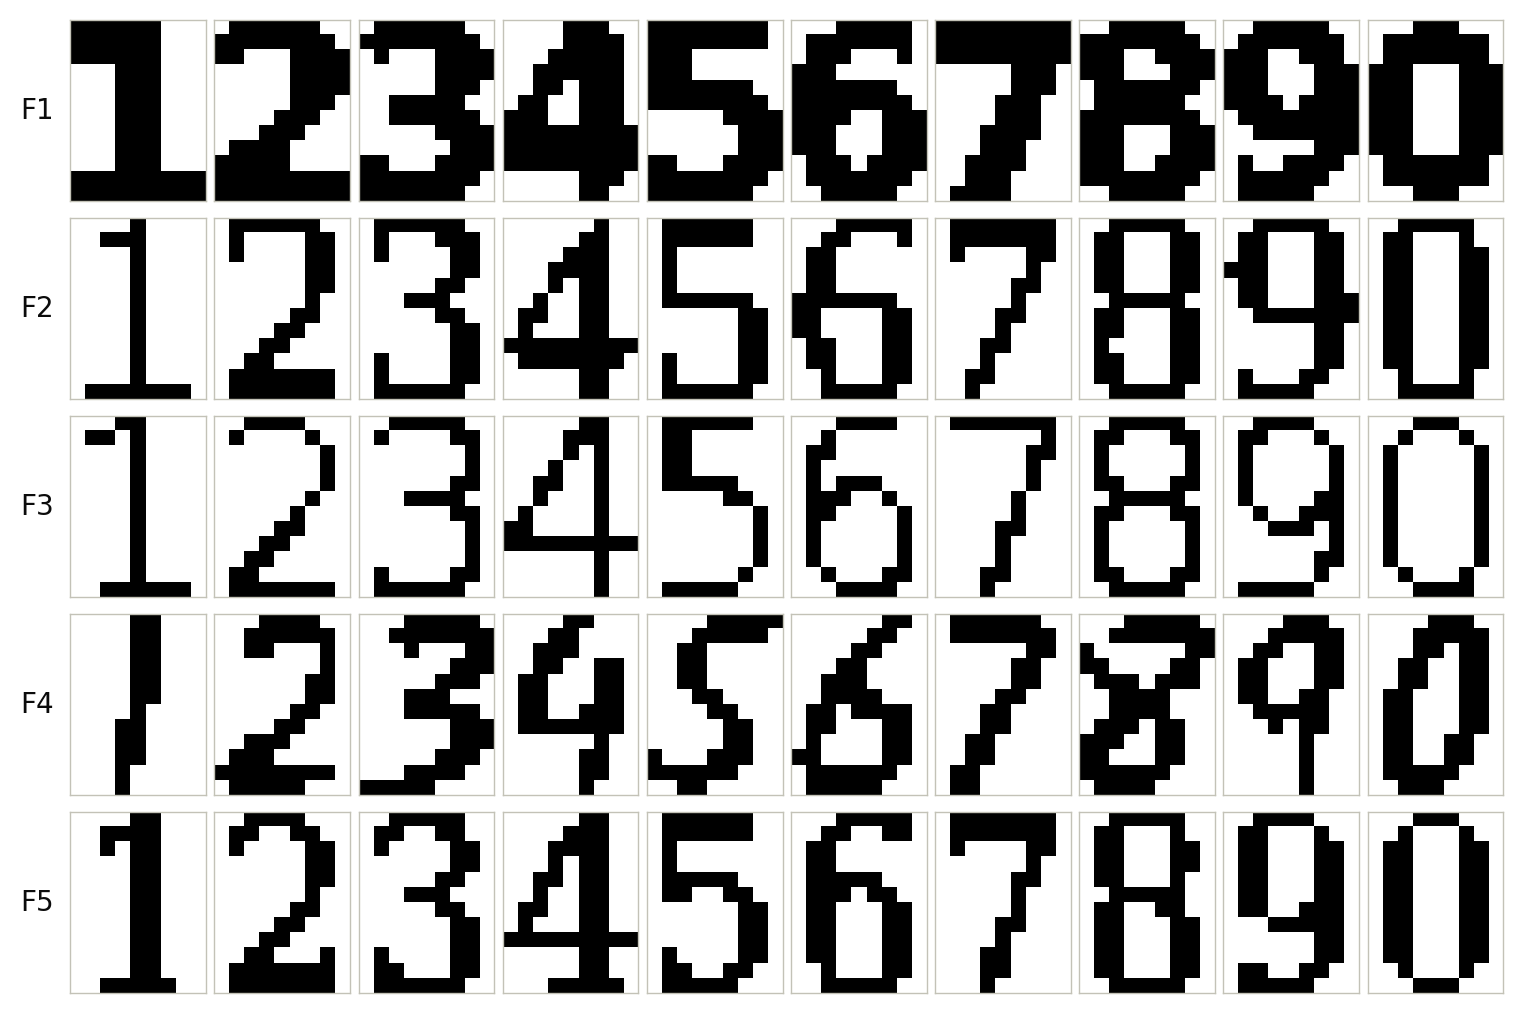
\includegraphics[width=0.66\textwidth]{fig_base_dados.png}
  \fonte{elaborada pelo autor (2026).}
\end{figure}

As versões ruidosas invertem o sinal de uma fração exata dos 108 pixels de cada padrão
(5, 10, 15 e 20\%), em posições sorteadas com semente fixa.

\subsection{Arquitetura e hiperparâmetros}

A rede tem 108 entradas, uma camada oculta e 10 saídas com codificação bipolar
\textit{one-hot} ($+1$ na classe correta e $-1$ nas demais); a classe atribuída é a do
neurônio de maior saída. O treinamento é padrão a padrão, em ordem aleatória a cada época, e
para quando o erro quadrático total $E_{\text{total}}=\frac12\sum_p\sum_k(t_{pk}-y_{pk})^2$
fica abaixo da tolerância ou ao atingir o limite de épocas (Tabela~\ref{tab:hiper}).

\begin{table}[H]
  \centering
  \caption{Hiperparâmetros da MLP}
  \label{tab:hiper}
  \begin{tabular}{lc}
    \toprule
    Parâmetro & Valor \\
    \midrule
    Neurônios ocultos & 20 \\
    Taxa de aprendizagem $\alpha$ & 0,01 \\
    Momento $\mu$ & 0,8 \\
    Tolerância de $E_{\text{total}}$ & 0,05 \\
    Máximo de épocas & 5000 \\
    Pesos iniciais & $U(-0{,}1;\;0{,}1)$, semente 2026 \\
    \bottomrule
  \end{tabular}
  \fonte{elaborada pelo autor (2026).}
\end{table}

A amplitude dos pesos iniciais foi reduzida em relação ao valor usual de $\pm0{,}5$: com 108
entradas bipolares, essa amplitude leva a entrada líquida dos neurônios ocultos a valores
que saturam a $\tanh$ ($f'\approx 0$), e num ensaio preliminar a rede não convergiu. Toda a
implementação usa apenas NumPy \cite{harris2020} (Apêndice~A).

Nos experimentos de ruído, cada nível foi avaliado em 30 repetições sobre os 50 padrões.
No \textit{leave-one-font-out} e no estudo de sensibilidade, cada configuração foi treinada
com 5 inicializações (sementes 2026 a 2030).

\section{Resultados}

\subsection{Treinamento e matriz de confusão}

O erro quadrático total caiu de 76,24 na primeira época para 0,0498 na época 144, quando o
critério de parada foi atingido (Figura~\ref{fig:erro}). Sem o termo de momento, a mesma
rede, com a mesma inicialização, precisou de 663 épocas. Nos dois casos a acurácia de treino
foi de 100,0\%, e a matriz de confusão de treino é diagonal
(Figura~\ref{fig:confusao}, à esquerda).

\begin{figure}[H]
  \centering
  \caption{Erro quadrático total por época (20 neurônios ocultos, com momento)}
  \label{fig:erro}
  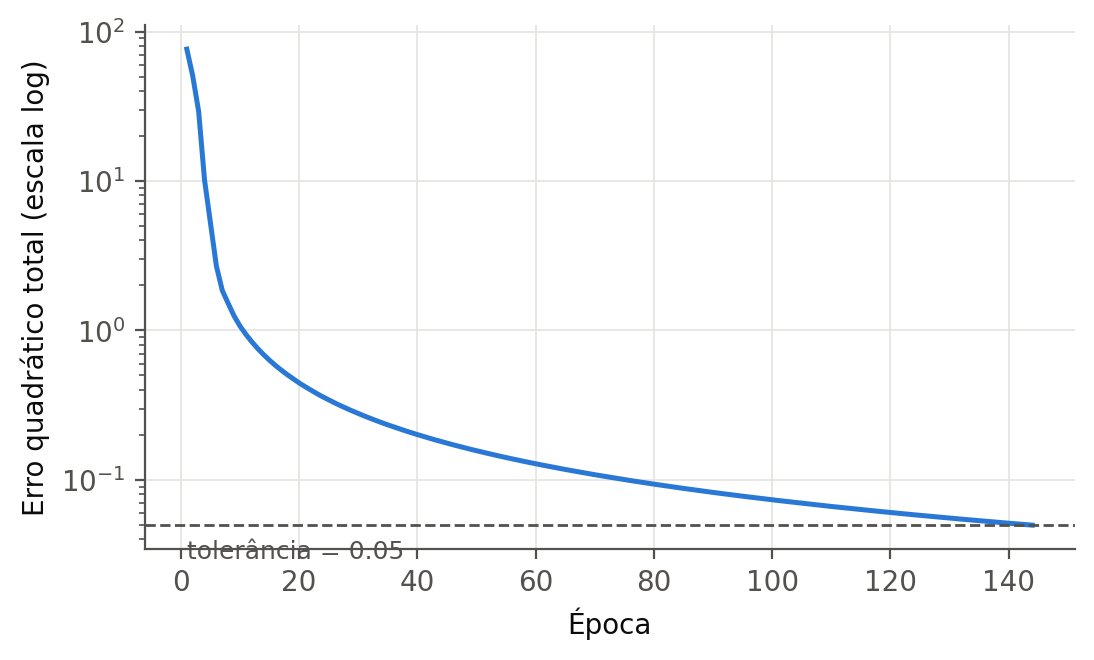
\includegraphics[width=0.66\textwidth]{fig_curva_erro.png}
  \fonte{elaborada pelo autor (2026).}
\end{figure}

\subsection{Robustez a ruído}

A acurácia permaneceu em 100,0\% com 5\% e 10\% de pixels invertidos, caiu para 98,9\%
(desvio padrão de 1,3 ponto) com 15\% e para 94,5\% (desvio de 3,5) com 20\%
(Figura~\ref{fig:ruido}). Com 10\% de ruído, a acurácia foi de 100,0\% em cada uma das
cinco fontes. A matriz acumulada sob 20\% de ruído (Figura~\ref{fig:confusao}, à direita)
mostra que o dígito 8 é o mais afetado: 128 acertos em 150, com confusões principalmente
para 0 (9 casos) e 6 (7 casos); em seguida aparece a troca de 3 por 8 (6 casos).

\begin{figure}[H]
  \centering
  \caption{Acurácia média em função do nível de ruído (faixa: $\pm$ 1 desvio padrão, 30 repetições)}
  \label{fig:ruido}
  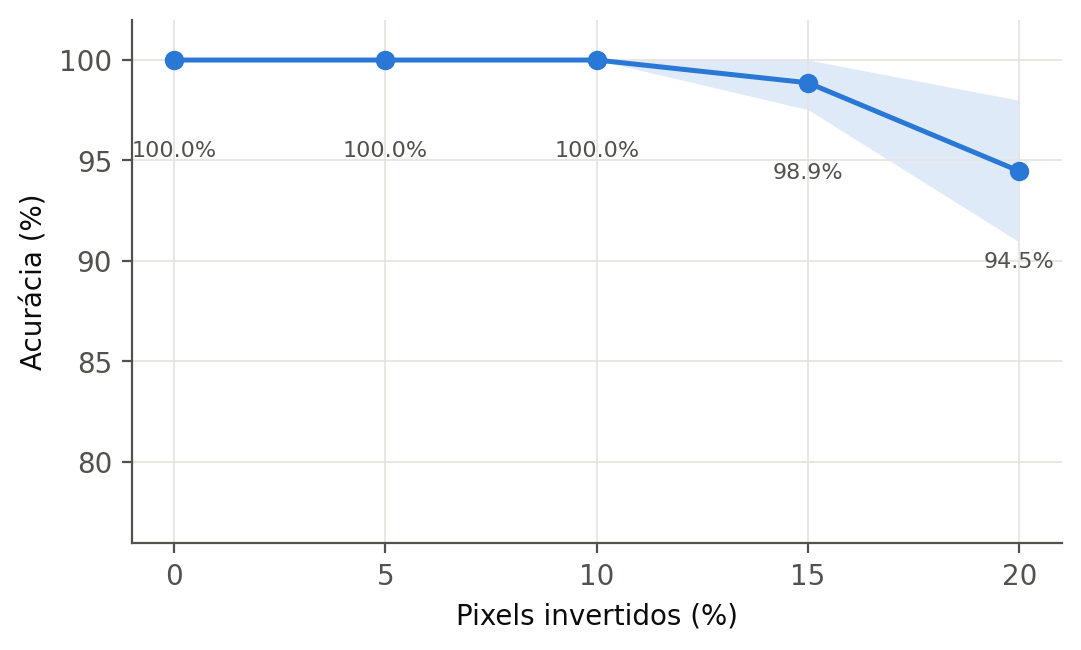
\includegraphics[width=0.66\textwidth]{fig_ruido.png}
  \fonte{elaborada pelo autor (2026).}
\end{figure}

\begin{figure}[H]
  \centering
  \caption{Matrizes de confusão: treino sem ruído e com 20\% de ruído (30 repetições acumuladas)}
  \label{fig:confusao}
  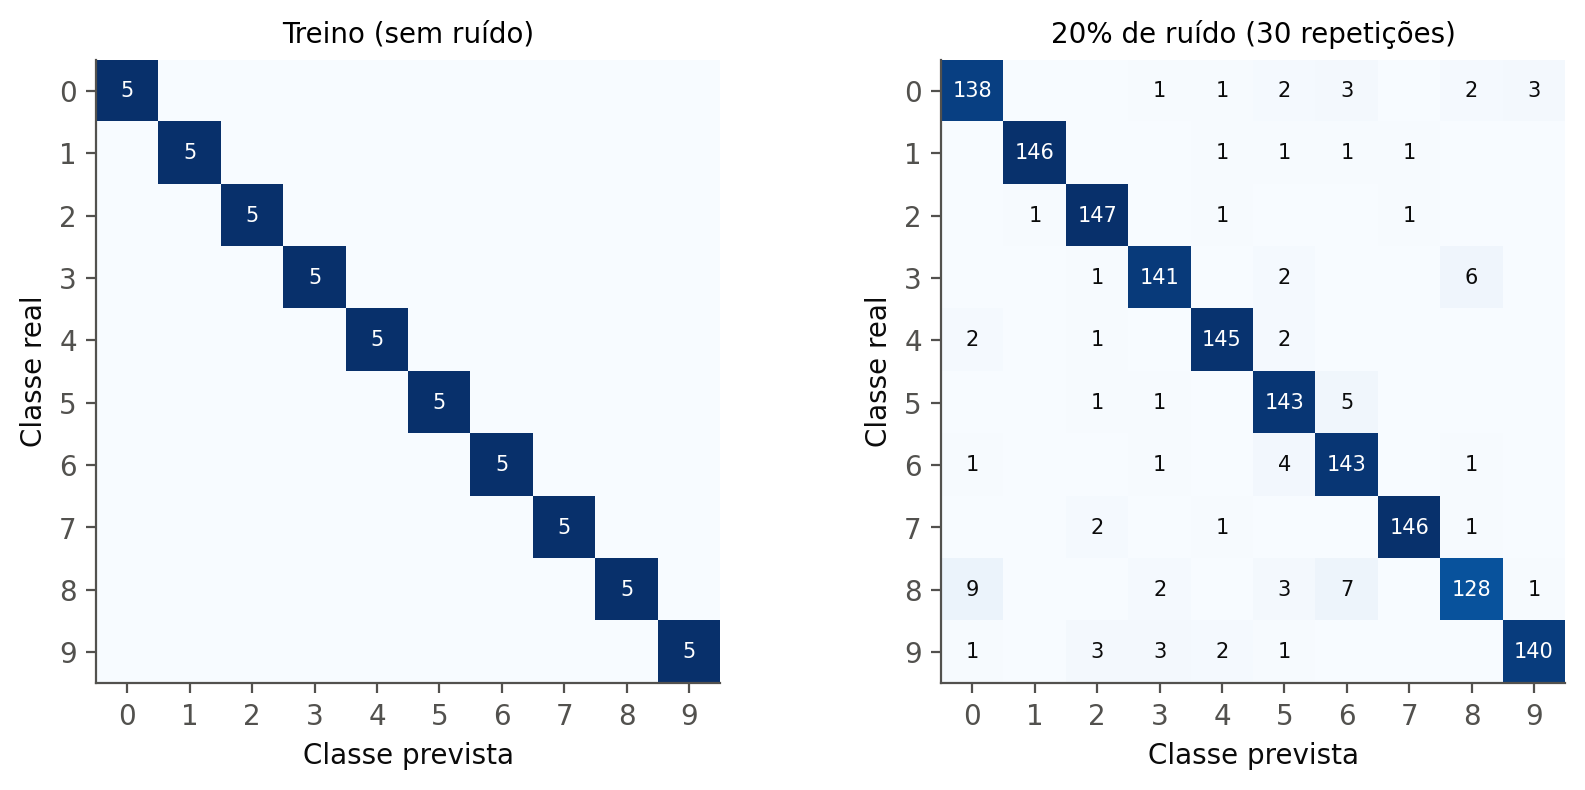
\includegraphics[width=0.85\textwidth]{fig_confusao.png}
  \fonte{elaborada pelo autor (2026).}
\end{figure}

\subsection{Generalização entre fontes}

A Tabela~\ref{tab:lofo} resume o teste \textit{leave-one-font-out}. As três fontes
serifadas ou finas foram reconhecidas integralmente quando deixadas de fora; a negrito teve
94,0\% e a manuscrita, 62,0\%. A média geral foi de 91,2\%. Os treinos com 40 padrões
convergiram, em média, entre 137,6 e 144,0 épocas, conforme a fonte excluída.

\begin{table}[H]
  \centering
  \caption{Acurácia na fonte excluída do treino (média $\pm$ desvio de 5 inicializações)}
  \label{tab:lofo}
  \begin{tabular}{llc}
    \toprule
    Fonte de teste & Erros (semente 2026) & Acurácia (\%) \\
    \midrule
    F1 -- sem serifa negrito     & --- & $94{,}0 \pm 8{,}0$ \\
    F2 -- serifada regular       & --- & $100{,}0 \pm 0{,}0$ \\
    F3 -- sem serifa fina        & --- & $100{,}0 \pm 0{,}0$ \\
    F4 -- manuscrita             & $4\!\to\!9$, $5\!\to\!7$, $6\!\to\!8$ & $62{,}0 \pm 7{,}5$ \\
    F5 -- serifada condensada    & --- & $100{,}0 \pm 0{,}0$ \\
    \midrule
    Média geral & & $91{,}2$ \\
    \bottomrule
  \end{tabular}
  \fonte{elaborada pelo autor (2026).}
\end{table}

\subsection{Sensibilidade ao número de neurônios ocultos}

Com 5 neurônios ocultos, apenas 2 das 5 inicializações atingiram a tolerância antes de 5000
épocas; a acurácia média de treino foi de 91,6\% e, com 10\% de ruído, de 85,0\%. A partir
de 10 neurônios todas as inicializações convergiram, e o número de épocas caiu à medida que
a camada oculta cresceu (Tabela~\ref{tab:sens}).

\begin{table}[H]
  \centering
  \caption{Efeito do número de neurônios ocultos (média de 5 inicializações)}
  \label{tab:sens}
  \begin{tabular}{cccc}
    \toprule
    Ocultos & Épocas & Convergiram & Acurácia com 10\% de ruído (\%) \\
    \midrule
    5  & 3469,0 & 2/5 & 85,0 \\
    10 & 330,6  & 5/5 & 99,2 \\
    20 & 144,6  & 5/5 & 99,9 \\
    40 & 81,4   & 5/5 & 99,9 \\
    \bottomrule
  \end{tabular}
  \fonte{elaborada pelo autor (2026).}
\end{table}

\section{Discussão}

A rede memoriza com facilidade os 50 padrões, e o momento reduziu as épocas de treinamento
em cerca de 4,6 vezes (663 contra 144), o que ilustra seu papel de acumular a direção
consistente do gradiente \cite{haykin2009}. A robustez a ruído é alta porque, em 108
pixels, inverter 10\% ainda deixa o padrão mais próximo do seu protótipo do que dos
demais; as falhas com 20\% de ruído concentram-se em pares que compartilham traços na
grade $12\times9$ (8, 0 e 6; 3 e 8; 5 e 6).

A generalização entre fontes revela o limite de uma base tão pequena. As fontes F2, F3 e F5
têm formas parecidas depois da redução para $12\times9$, de modo que qualquer uma delas é
bem representada pelas demais. A negrito ocupa em média 67 pixels, contra cerca de 40 nas
outras, e por isso depende mais da inicialização (desvio de 8 pontos). A manuscrita é a
mais distante: o 4 aberto, o 5 e o 6 inclinados e o 1 sem base não têm correspondentes no
treino, e com um único exemplo por fonte a rede não tem como aprender essa variação. Em
problemas reais, isso se resolve com muito mais exemplos por classe e, em geral, com
arquiteturas que exploram a estrutura espacial da imagem \cite{lecun1998}.

Quanto ao tamanho da camada oculta, 5 neurônios formam um gargalo: a rede fica presa em
mínimos em que algumas classes não se separam. De 10 em diante, mais neurônios aceleram o
treino, mas a robustez com 10\% de ruído praticamente não muda (99,2\% a 99,9\%). Os 20
neurônios adotados equilibram convergência rápida e tamanho da rede.

\section{Conclusão}

Foi construída uma base de 50 dígitos em cinco fontes e treinada uma MLP implementada do
zero. A rede convergiu em 144 épocas, reconheceu todos os padrões de treino e manteve
94,5\% de acurácia com 20\% dos pixels invertidos. A principal limitação apareceu no teste
entre fontes: 91,2\% de acurácia média, com apenas 62,0\% na fonte manuscrita, o que
mostra que cinco exemplos por classe bastam para memorizar e tolerar ruído, mas não para
generalizar para um estilo de escrita diferente. Como continuidade, seria possível ampliar
a base com mais fontes e com pequenas translações e rotações dos dígitos existentes.

%========================== REFERÊNCIAS ==============================
\newpage
\pagestyle{abnt}
\begin{singlespace}
\bibliography{referencias}
\end{singlespace}

%=========================== APÊNDICE ================================
\newpage
\appendix
\renewcommand{\thesection}{\Alph{section}}
\section*{APÊNDICE A -- CÓDIGO-FONTE EM PYTHON}
\addcontentsline{toc}{section}{APÊNDICE A -- CÓDIGO-FONTE EM PYTHON}
\noindent Arquivo \texttt{trabalho07\_digitos.py}, executado com
\texttt{python trabalho07\_digitos.py}.
\begin{singlespace}
\lstinputlisting{trabalho07_digitos.py}
\end{singlespace}

\end{document}
